\chapter{Additional Graphics}
\label{app:addional_graphics}


\begin{figure}[htb!]
    \centering
    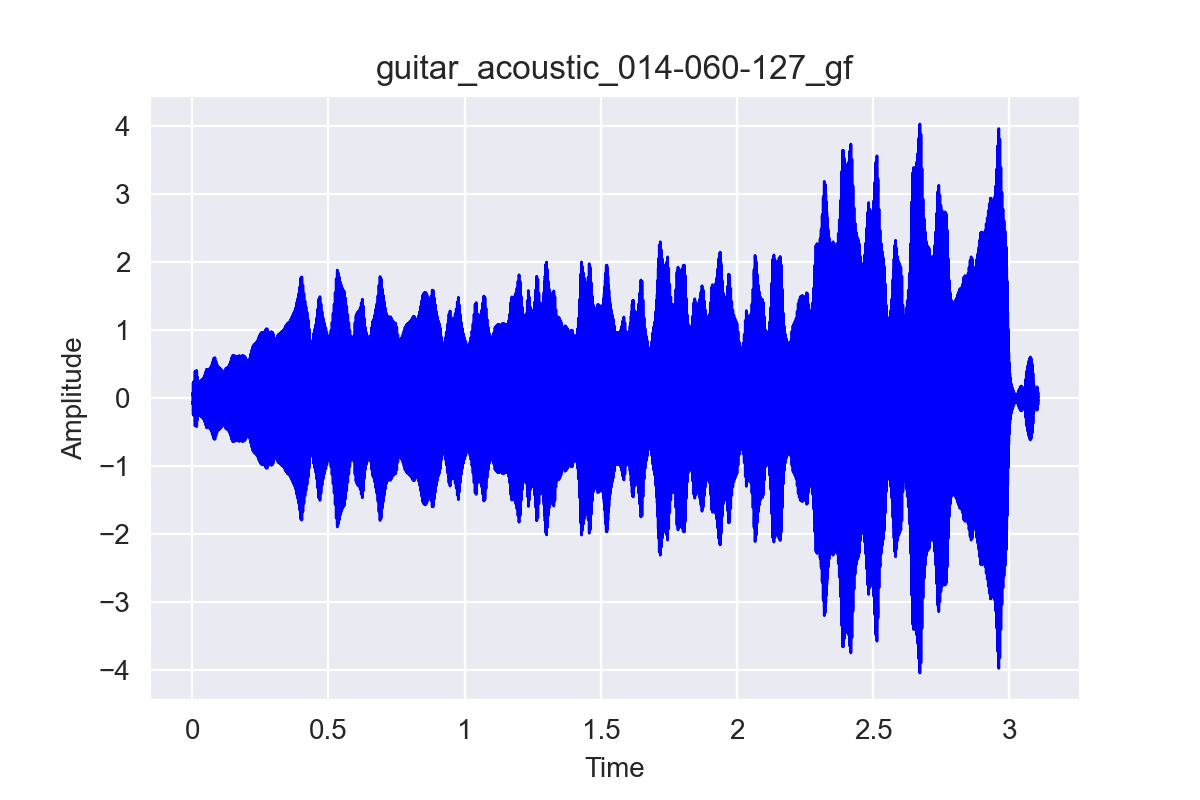
\includegraphics[width=0.55\textwidth]{images/appendix/1D/guitar_acoustic_014-060-127_gf.png}
    \caption{guitar acoustic output with griffin lim (1D conv).}
    \label{fig:res_2D_mel_guit}
\end{figure}


\begin{figure}[htb!]
    \centering
    \captionsetup{justification=centering}
    \makebox[\textwidth][c]{\begin{tabular}{@{}cc@{}}
        \makebox{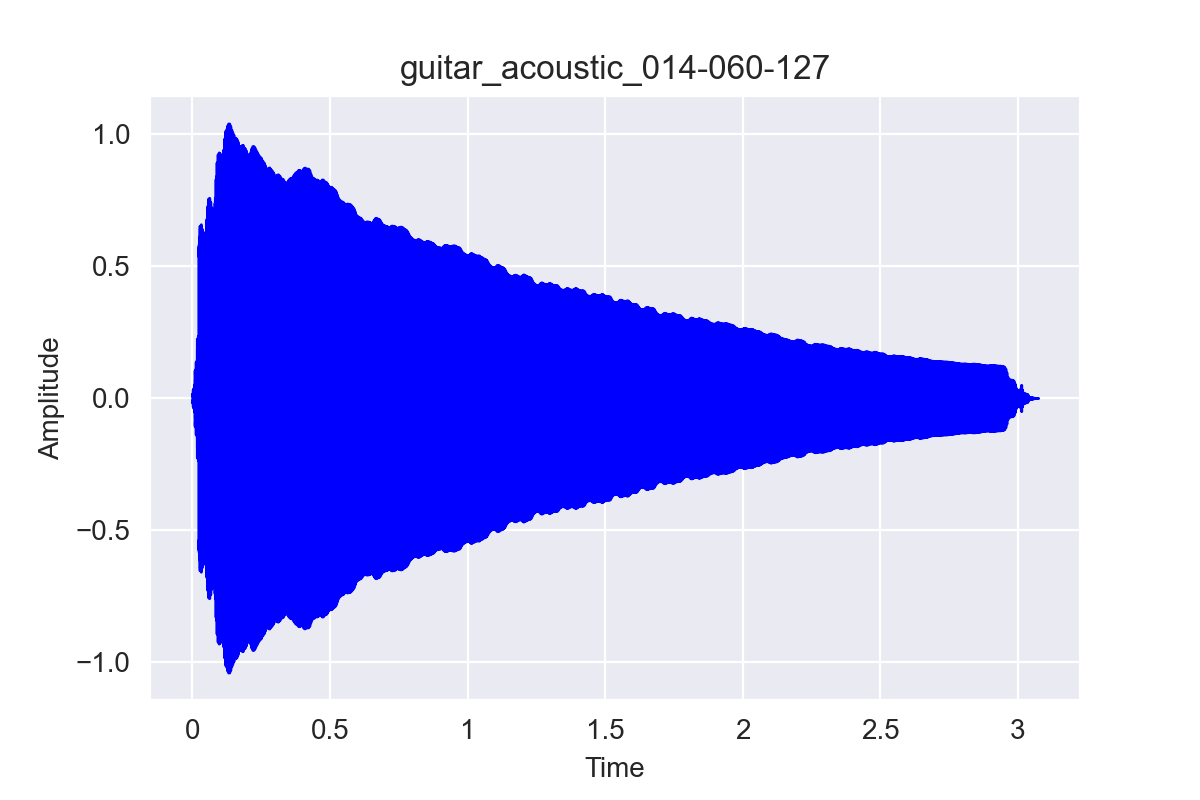
\includegraphics[width=0.55\textwidth]{images/appendix/single_stride/guitar_acoustic_014-060-127.png}}&
        \makebox{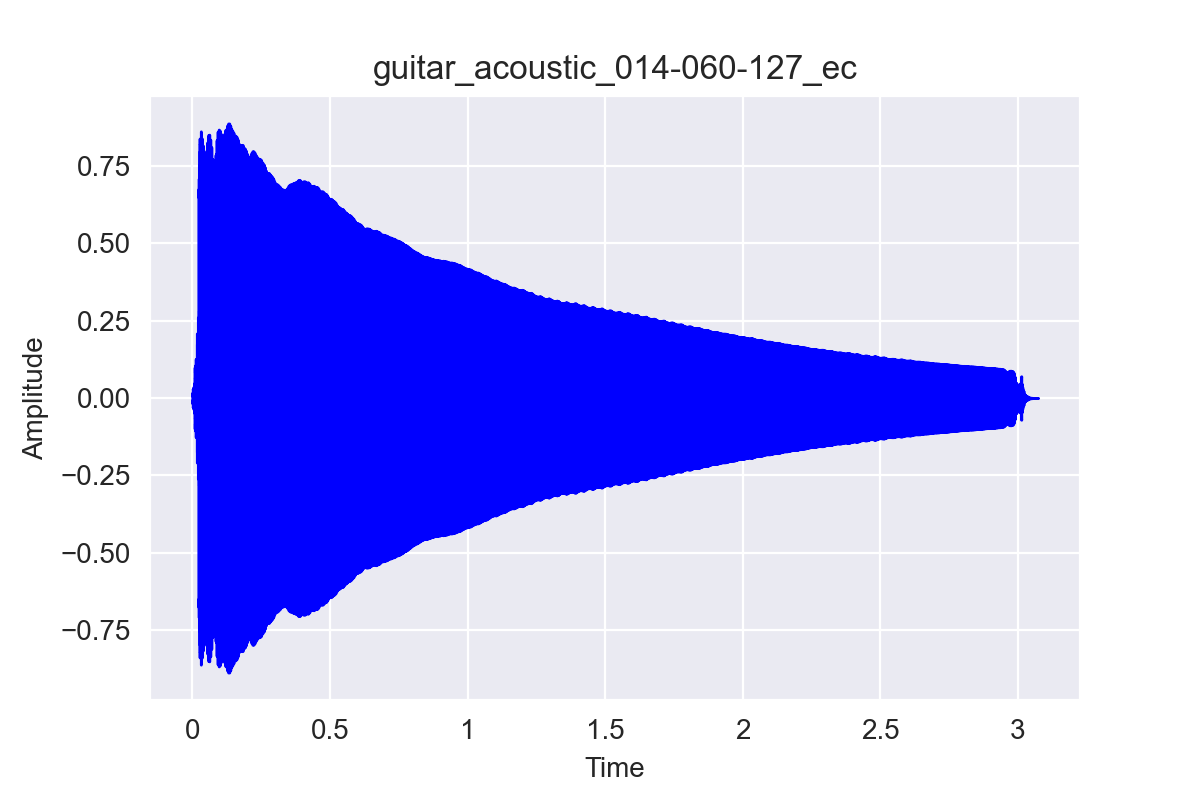
\includegraphics[width=0.55\textwidth]{images/appendix/single_stride/guitar_acoustic_014-060-127_ec.png}}\\
        (a) & (b)
    \end{tabular}}
    \caption{2D convolutional single-stride network - guitar acoustic output without post processing ~(a), output with post processing ~(b).}
    \label{fig:apx_single_phase}
\end{figure}

\begin{figure}[htb!]
    \centering
    \captionsetup{justification=centering}
    \makebox[\textwidth][c]{\begin{tabular}{@{}cc@{}}
        \makebox{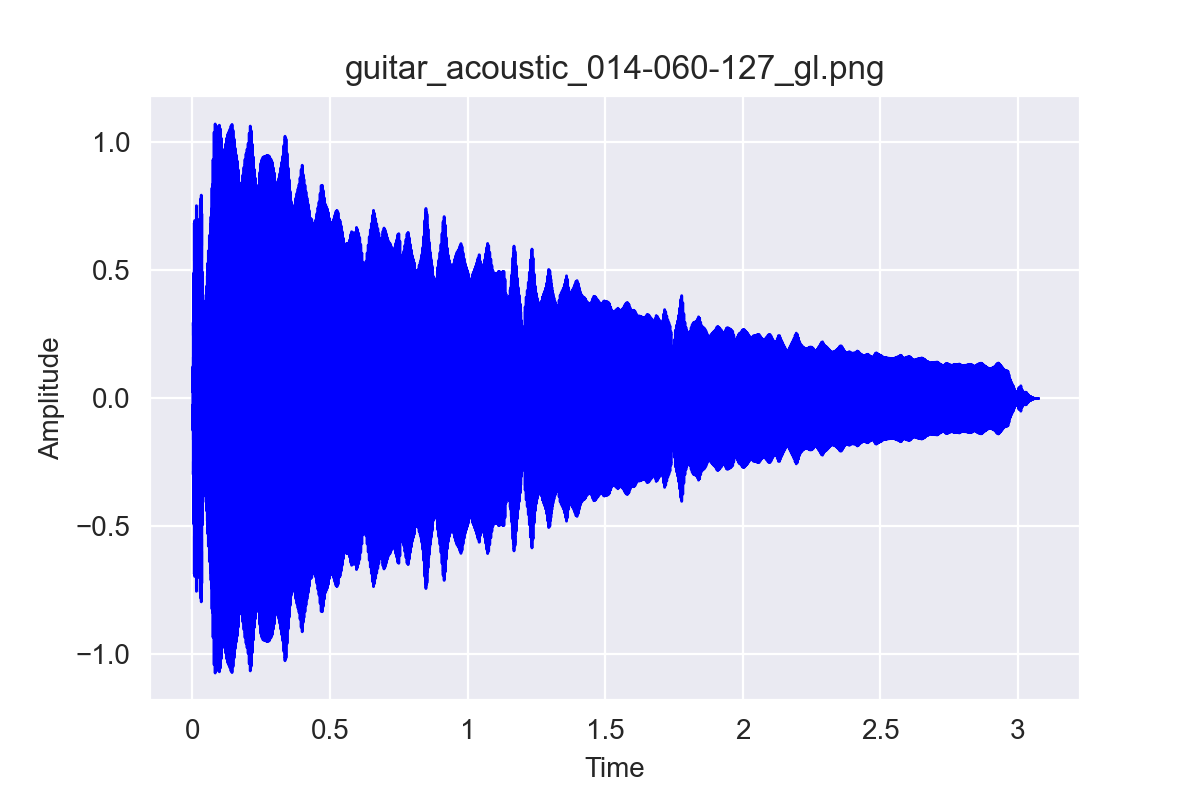
\includegraphics[width=0.55\textwidth]{images/appendix/single_stride/guitar_acoustic_014-060-127_gl.png}}&
        \makebox{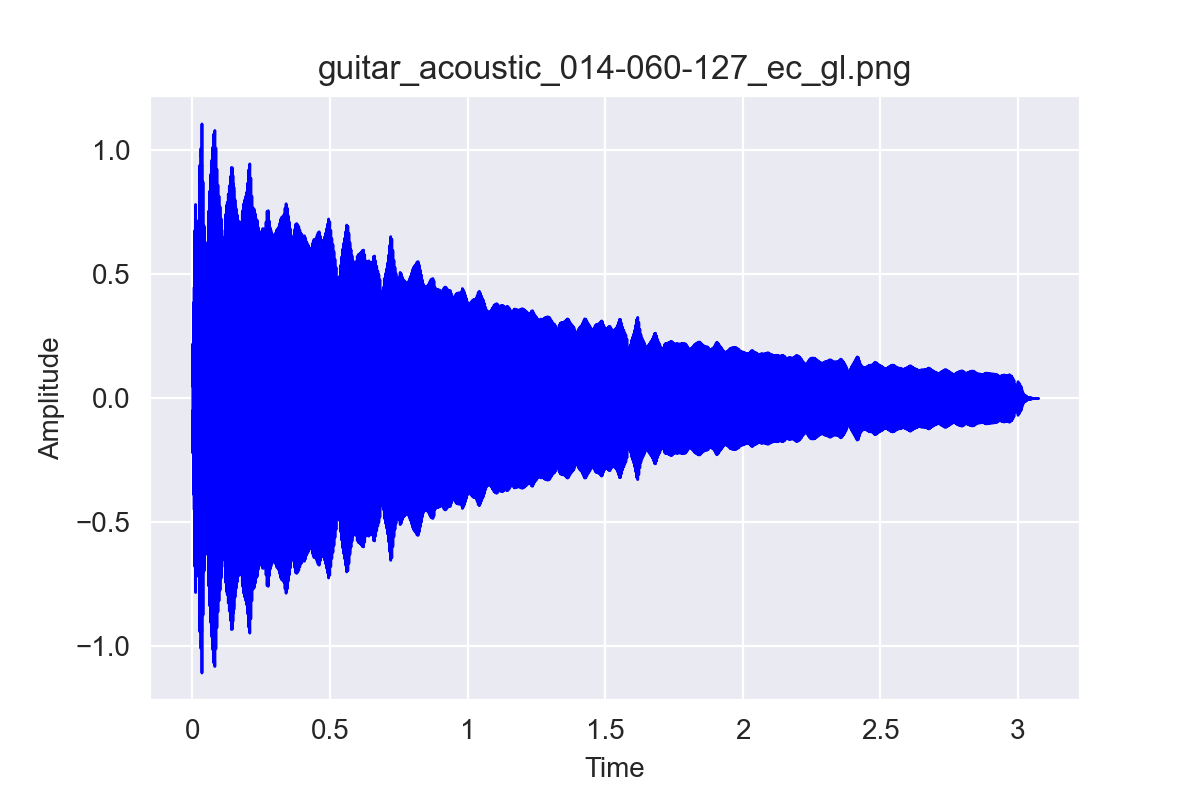
\includegraphics[width=0.55\textwidth]{images/appendix/single_stride/guitar_acoustic_014-060-127_ec_gl.png}}\\
        (a) & (b)
    \end{tabular}}
    \caption{2D convolutional single-stride network - guitar acoustic output without post processing and Griffin Lim ~(a), output with post processing and Griffin Lim ~(b).}
    \label{fig:apx_single_gf}
\end{figure}

\begin{figure}[htb!]
    \centering
    \captionsetup{justification=centering}
    \makebox[\textwidth][c]{\begin{tabular}{@{}cc@{}}
        \makebox{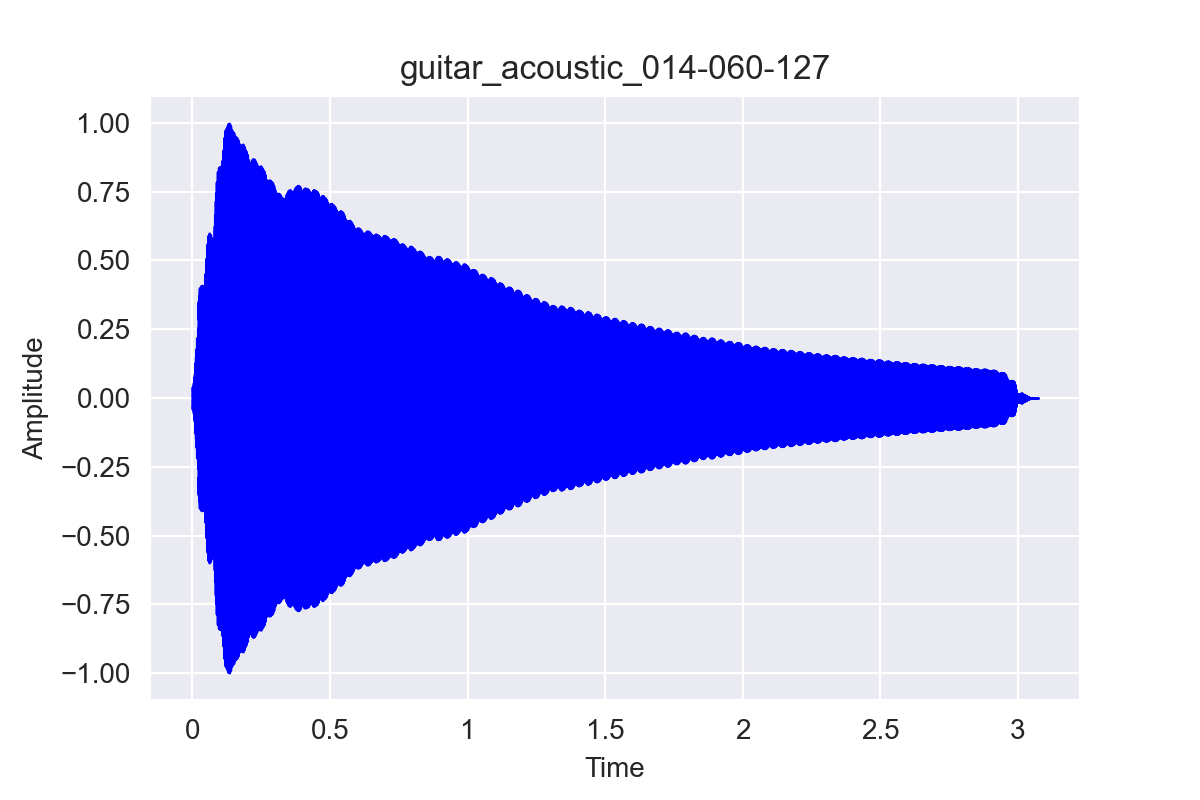
\includegraphics[width=0.55\textwidth]{images/appendix/double_stride/guitar_acoustic_014-060-127.png}}&
        \makebox{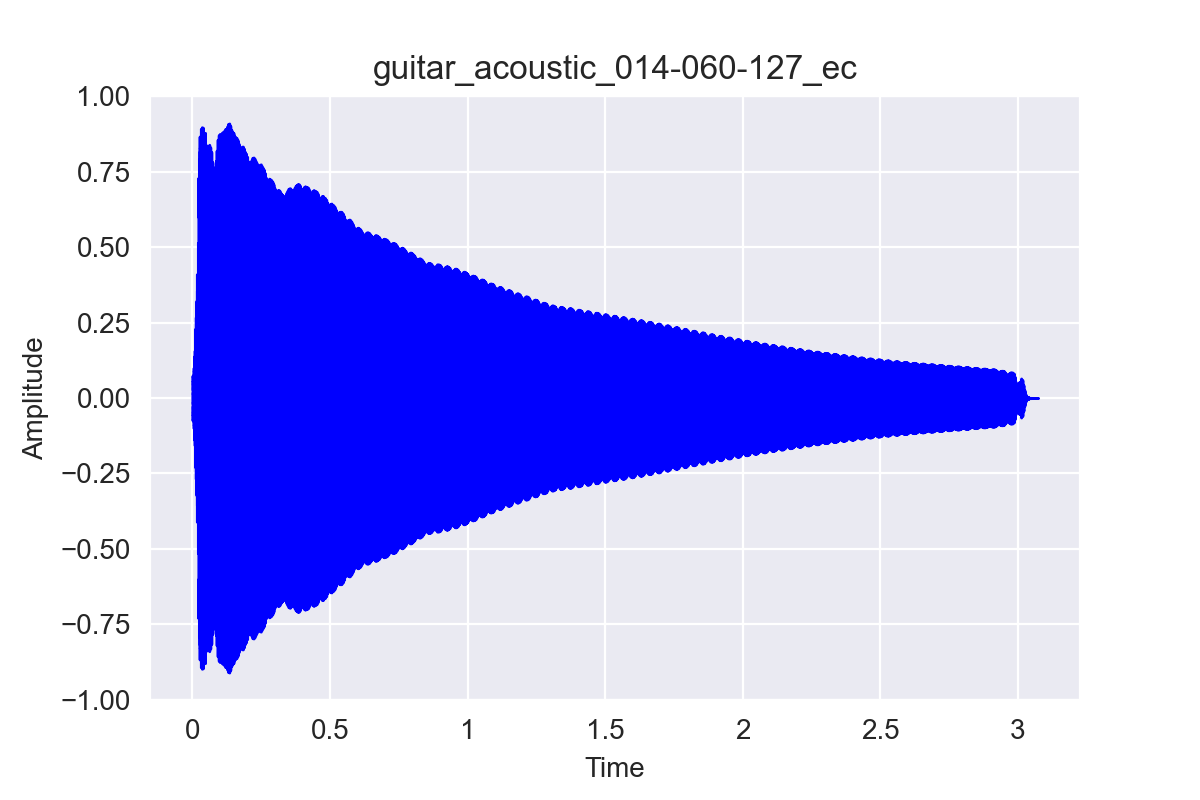
\includegraphics[width=0.55\textwidth]{images/appendix/double_stride/guitar_acoustic_014-060-127_ec.png}}\\
        (a) & (b)
    \end{tabular}}
    \caption{2D convolutional double-stride network - guitar acoustic output without post processing ~(a), output with post processing ~(b).}
    \label{fig:apx_double_phase}
\end{figure}

\begin{figure}[htb!]
    \centering
    \captionsetup{justification=centering}
    \makebox[\textwidth][c]{\begin{tabular}{@{}cc@{}}
        \makebox{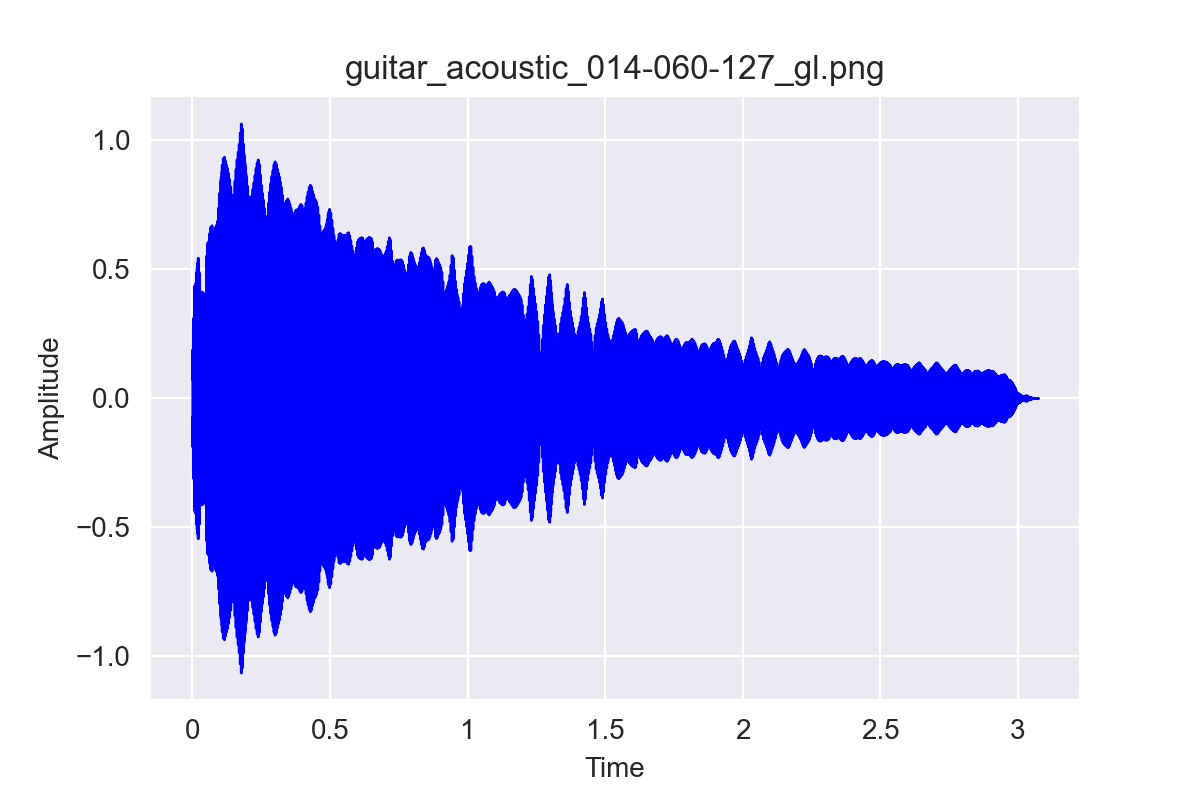
\includegraphics[width=0.55\textwidth]{images/appendix/double_stride/guitar_acoustic_014-060-127_gl.png}}&
        \makebox{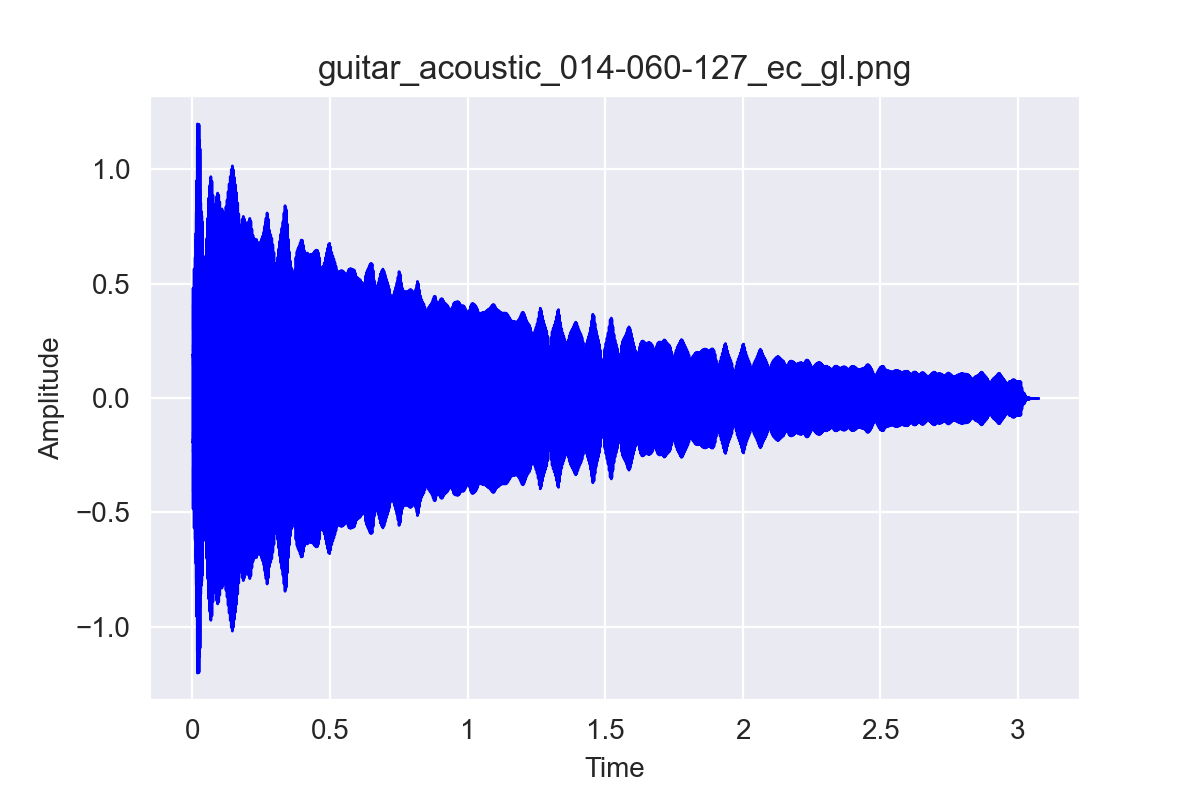
\includegraphics[width=0.55\textwidth]{images/appendix/double_stride/guitar_acoustic_014-060-127_ec_gl.png}}\\
        (a) & (b)
    \end{tabular}}
    \caption{2D convolutional double-stride network - guitar acoustic output without post processing and Griffin Lim ~(a), output with post processing and Griffin Lim ~(b).}
    \label{fig:apx_double_gf}
\end{figure}

\begin{figure}[htb!]
    \centering
    \captionsetup{justification=centering}
    \makebox[\textwidth][c]{\begin{tabular}{@{}cc@{}}
        \makebox{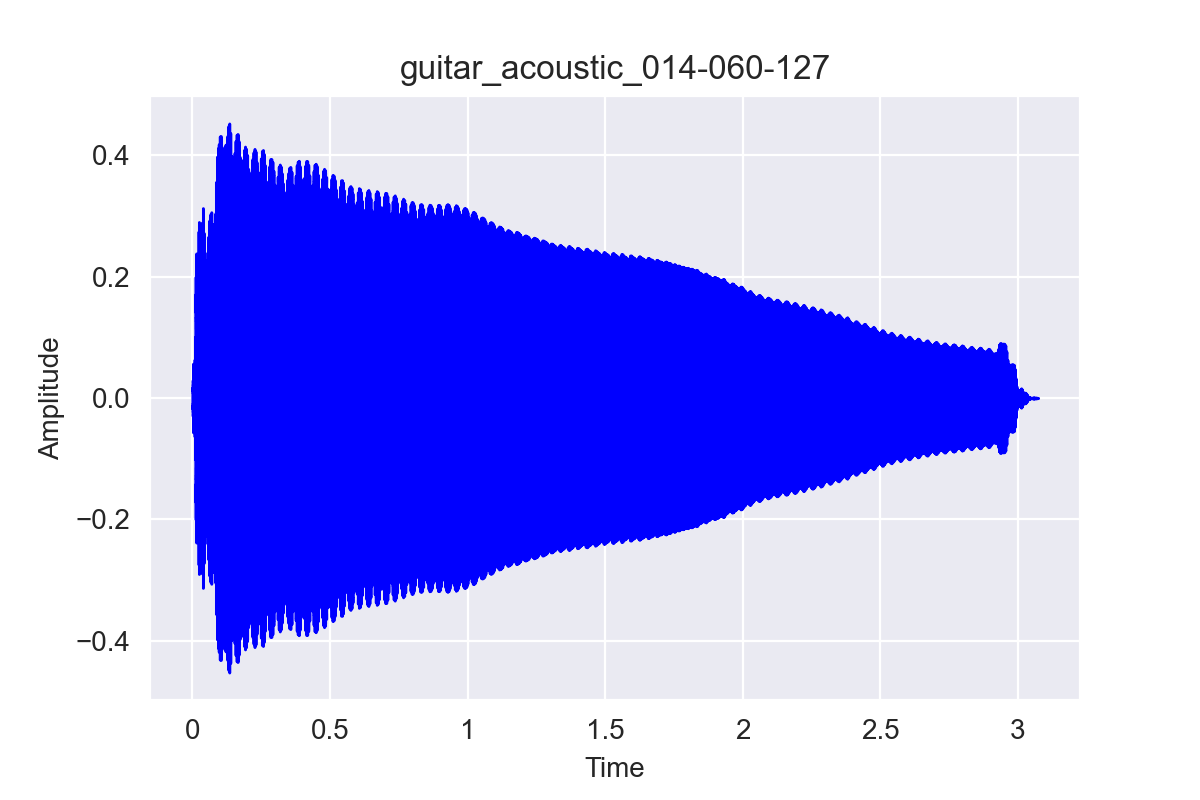
\includegraphics[width=0.55\textwidth]{images/appendix/triple_stride/guitar_acoustic_014-060-127.png}}&
        \makebox{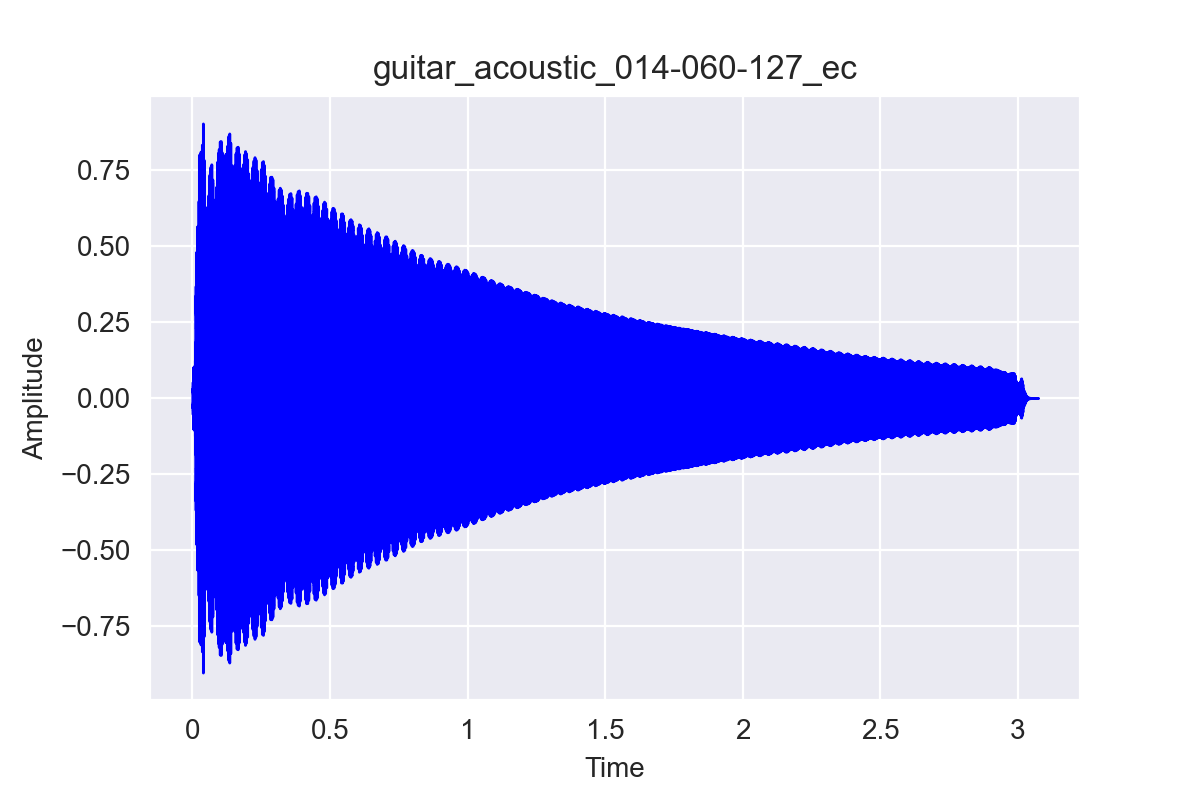
\includegraphics[width=0.55\textwidth]{images/appendix/triple_stride/guitar_acoustic_014-060-127_ec.png}}\\
        (a) & (b)
    \end{tabular}}
    \caption{2D convolutional triple-stride network - guitar acoustic output without post processing ~(a), output with post processing ~(b).}
    \label{fig:apx_triple_phase}
\end{figure}

\begin{figure}[htb!]
    \centering
    \captionsetup{justification=centering}
    \makebox[\textwidth][c]{\begin{tabular}{@{}cc@{}}
        \makebox{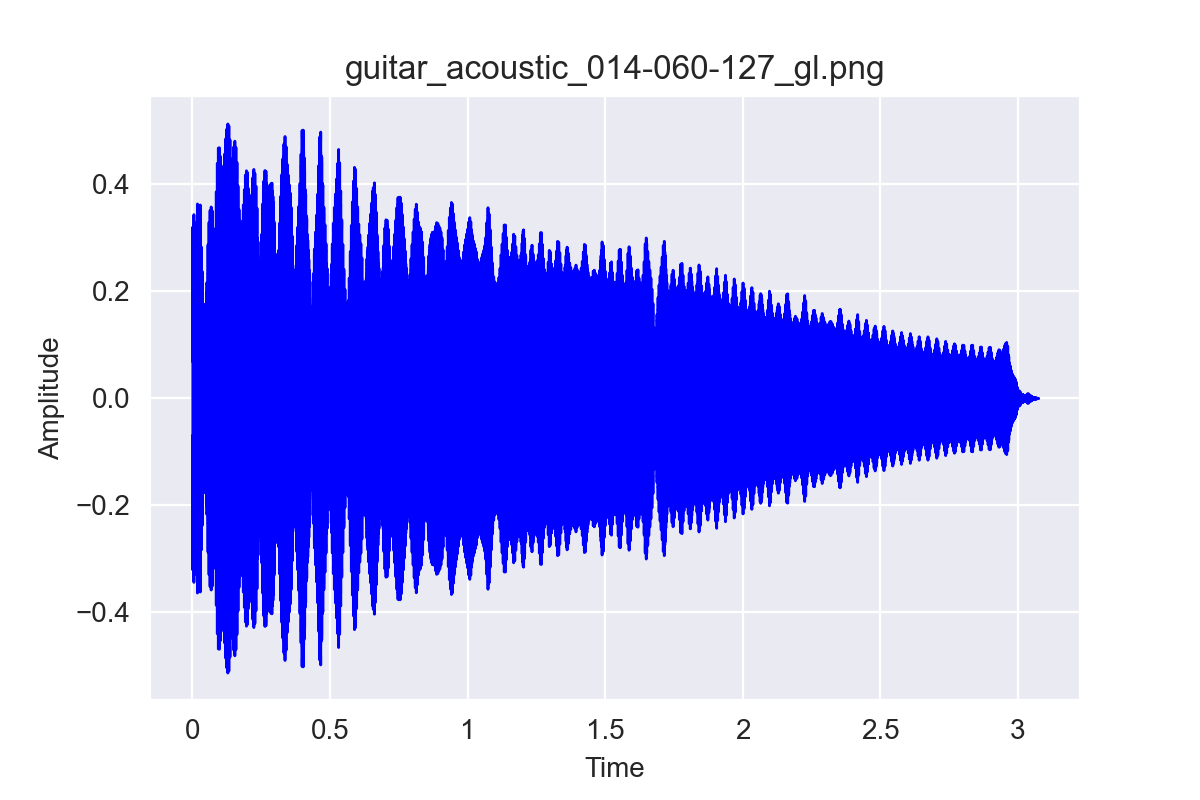
\includegraphics[width=0.55\textwidth]{images/appendix/triple_stride/guitar_acoustic_014-060-127_gl.png}}&
        \makebox{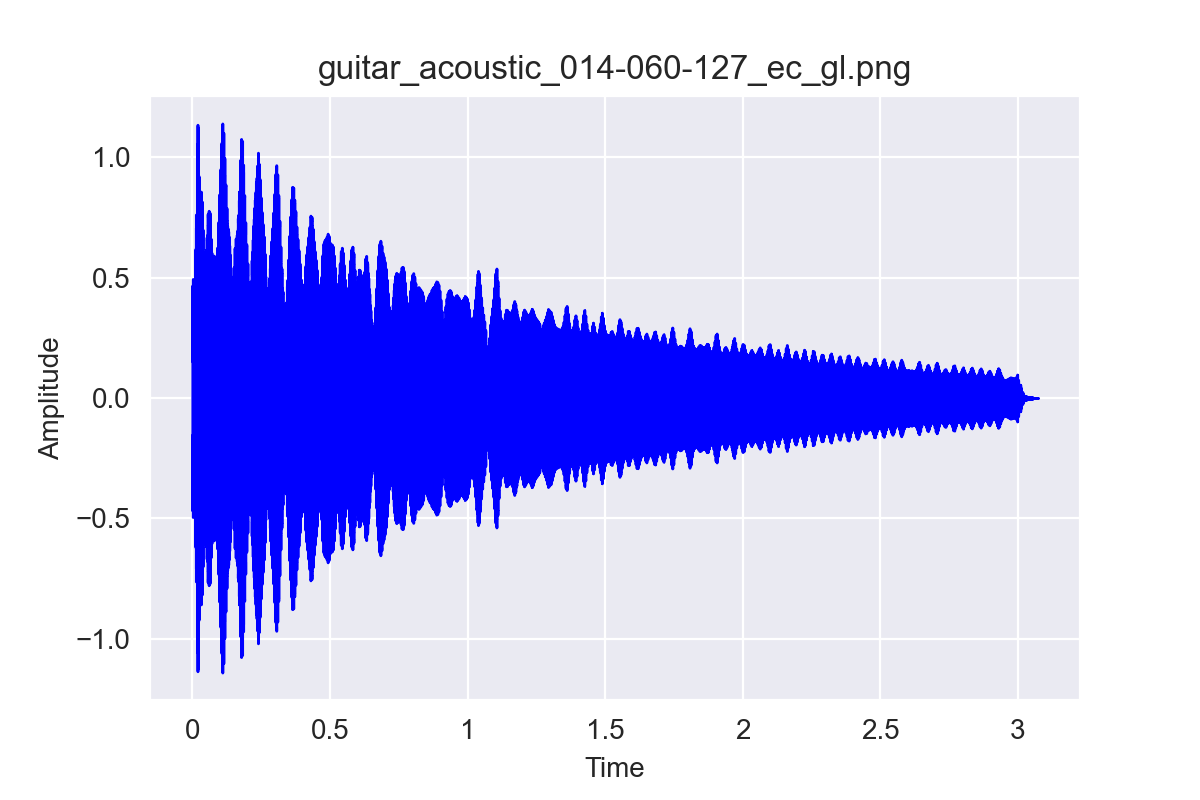
\includegraphics[width=0.55\textwidth]{images/appendix/triple_stride/guitar_acoustic_014-060-127_ec_gl.png}}\\
        (a) & (b)
    \end{tabular}}
    \caption{2D convolutional triple-stride network - guitar acoustic output without post processing and Griffin Lim ~(a), output with post processing and Griffin Lim ~(b).}
    \label{fig:apx_triple_gf}
\end{figure}


\begin{figure}[htb!]
    \centering
    \captionsetup{justification=centering}
    \makebox[\textwidth][c]{\begin{tabular}{@{}cc@{}}
        \makebox{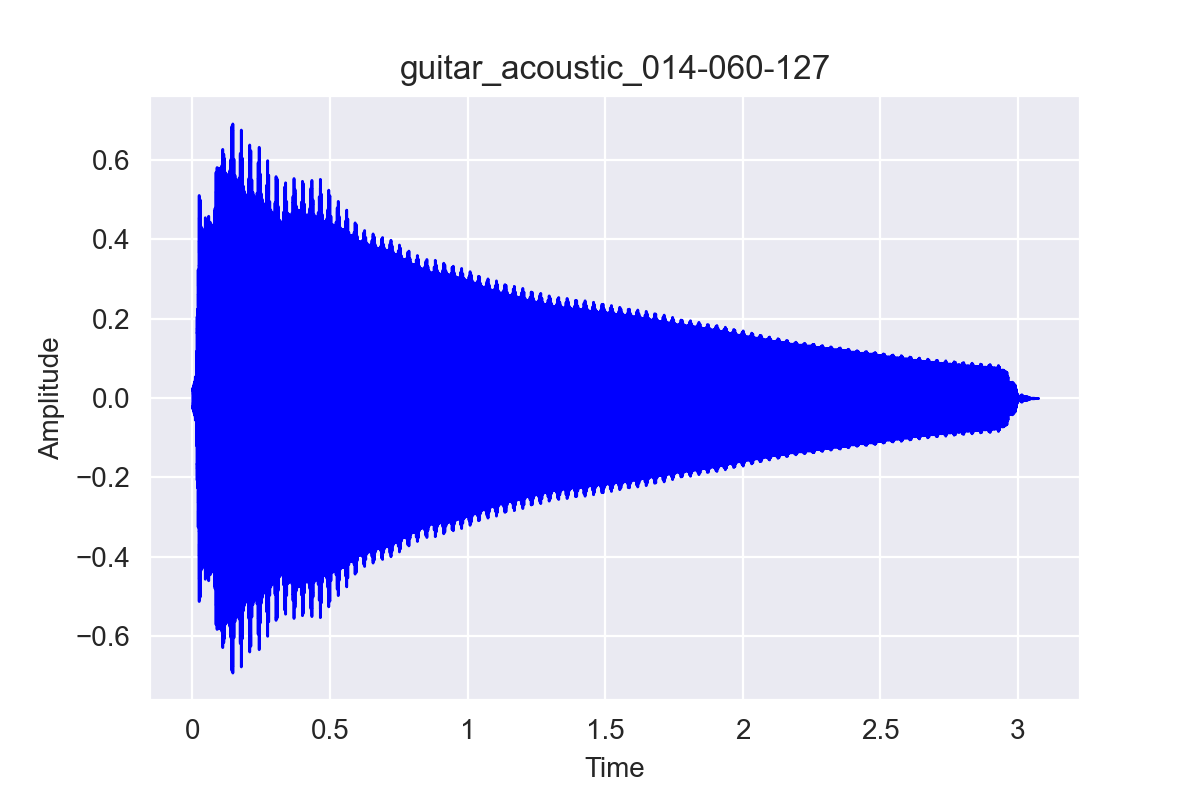
\includegraphics[width=0.55\textwidth]{images/appendix/mel_single_stride/guitar_acoustic_014-060-127.png}}&
        \makebox{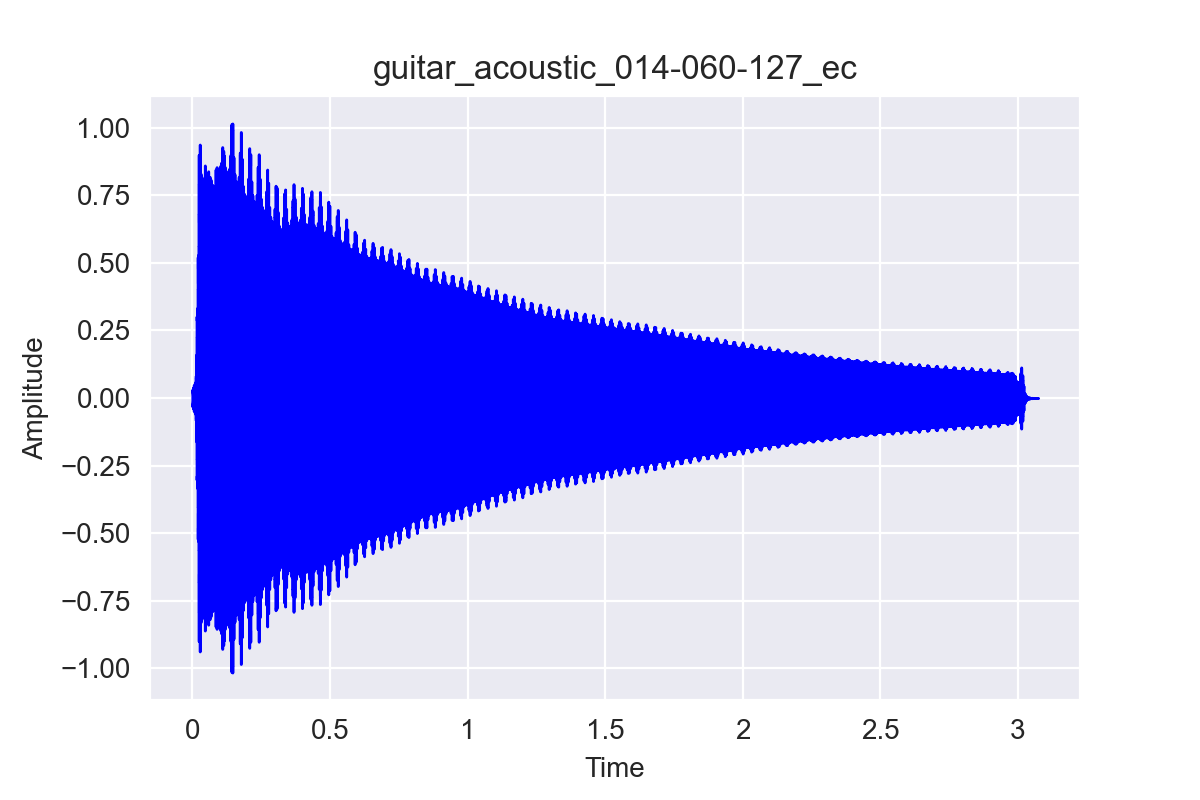
\includegraphics[width=0.55\textwidth]{images/appendix/mel_single_stride/guitar_acoustic_014-060-127_ec.png}}\\
        (a) & (b)
    \end{tabular}}
    \caption{2D convolutional single-stride network (log-mel) - guitar acoustic output without post processing ~(a), output with post processing ~(b).}
    \label{fig:apx_mel_single_phase}
\end{figure}

\begin{figure}[htb!]
    \centering
    \captionsetup{justification=centering}
    \makebox[\textwidth][c]{\begin{tabular}{@{}cc@{}}
        \makebox{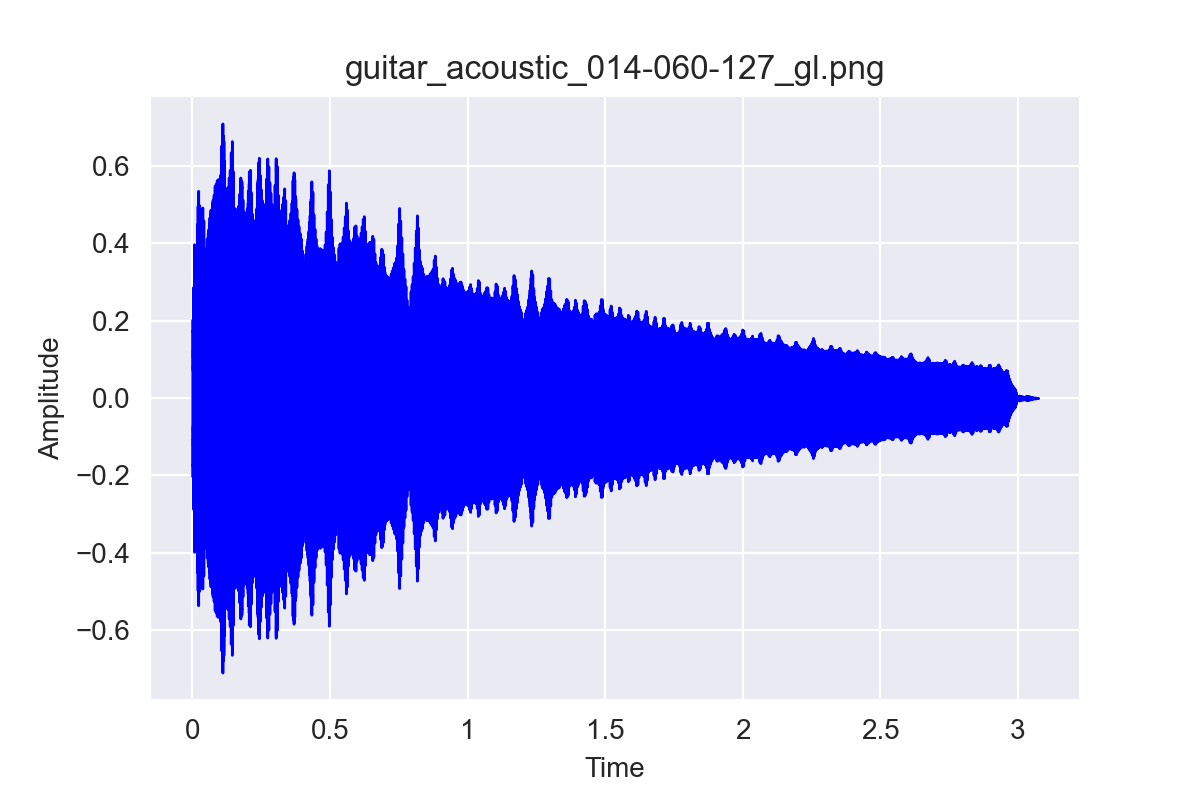
\includegraphics[width=0.55\textwidth]{images/appendix/mel_single_stride/guitar_acoustic_014-060-127_gl.png}}&
        \makebox{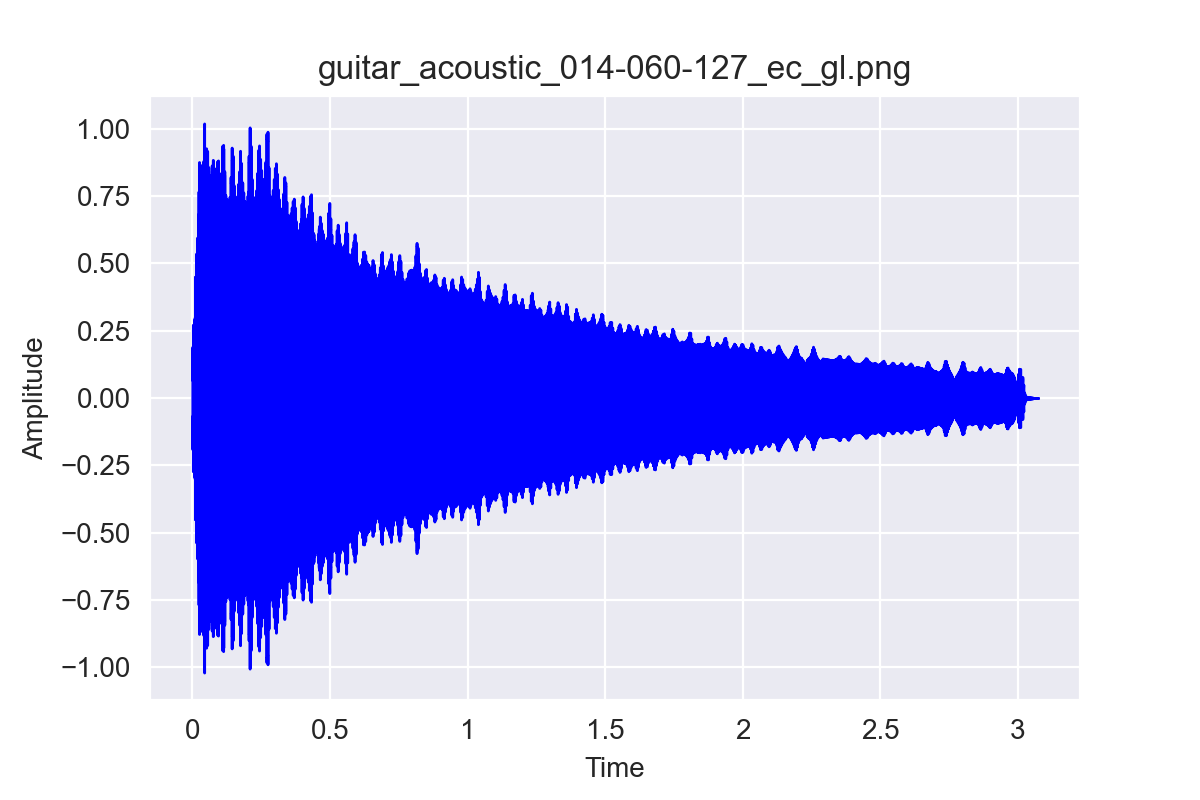
\includegraphics[width=0.55\textwidth]{images/appendix/mel_single_stride/guitar_acoustic_014-060-127_ec_gl.png}}\\
        (a) & (b)
    \end{tabular}}
    \caption{2D convolutional single-stride network (log-mel) - guitar acoustic output without post processing and Griffin Lim ~(a), output with post processing and Griffin Lim ~(b).}
    \label{fig:apx_mel_single_gf}
\end{figure}

\begin{figure}[htb!]
    \centering
    \captionsetup{justification=centering}
    \makebox[\textwidth][c]{\begin{tabular}{@{}cc@{}}
        \makebox{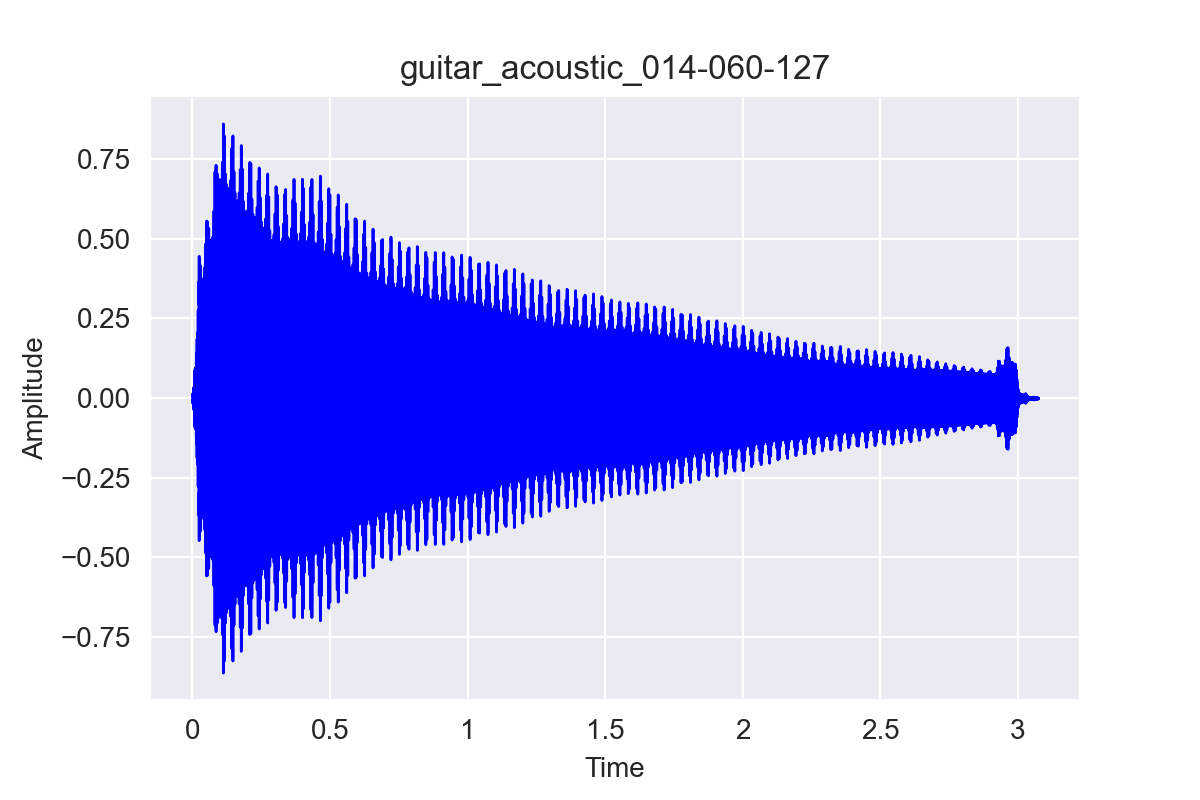
\includegraphics[width=0.55\textwidth]{images/appendix/mel_double_stride/guitar_acoustic_014-060-127.png}}&
        \makebox{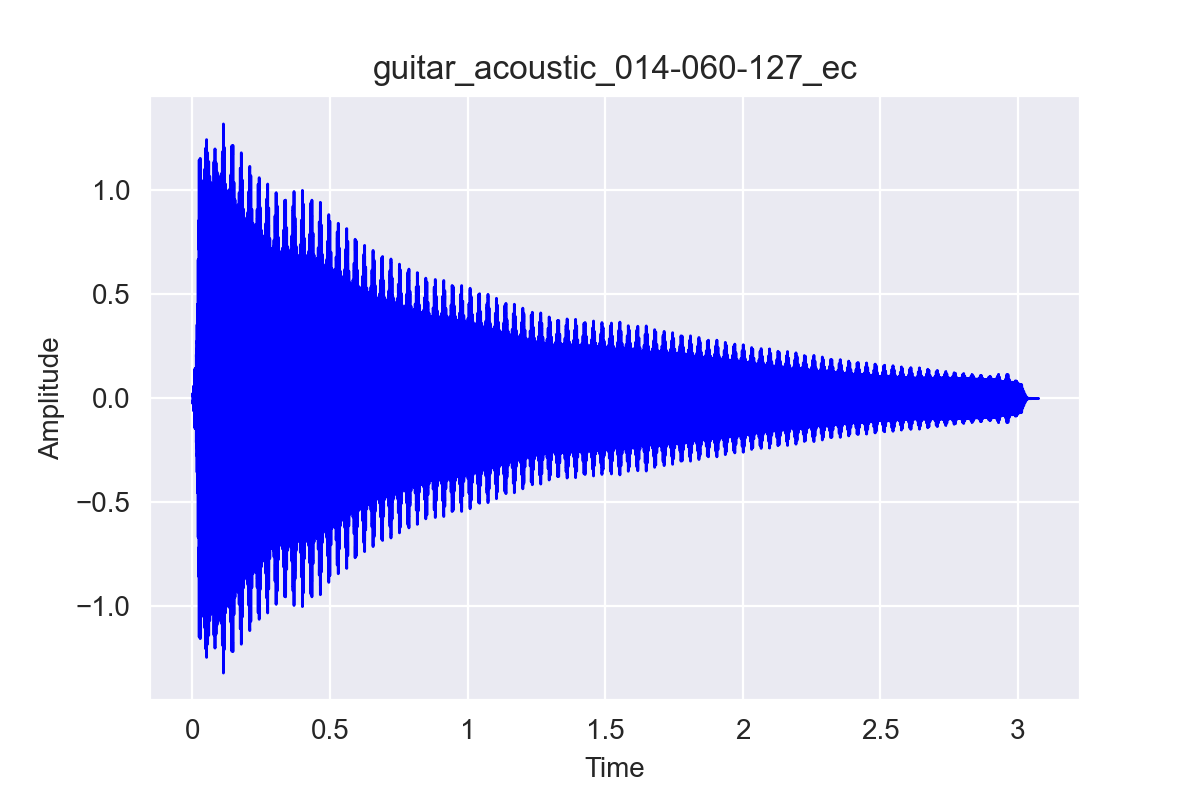
\includegraphics[width=0.55\textwidth]{images/appendix/mel_double_stride/guitar_acoustic_014-060-127_ec.png}}\\
        (a) & (b)
    \end{tabular}}
    \caption{2D convolutional double-stride network (log-mel) - guitar acoustic output without post processing ~(a), output with post processing ~(b).}
    \label{fig:apx_mel_double_phase}
\end{figure}

\begin{figure}[htb!]
    \centering
    \captionsetup{justification=centering}
    \makebox[\textwidth][c]{\begin{tabular}{@{}cc@{}}
        \makebox{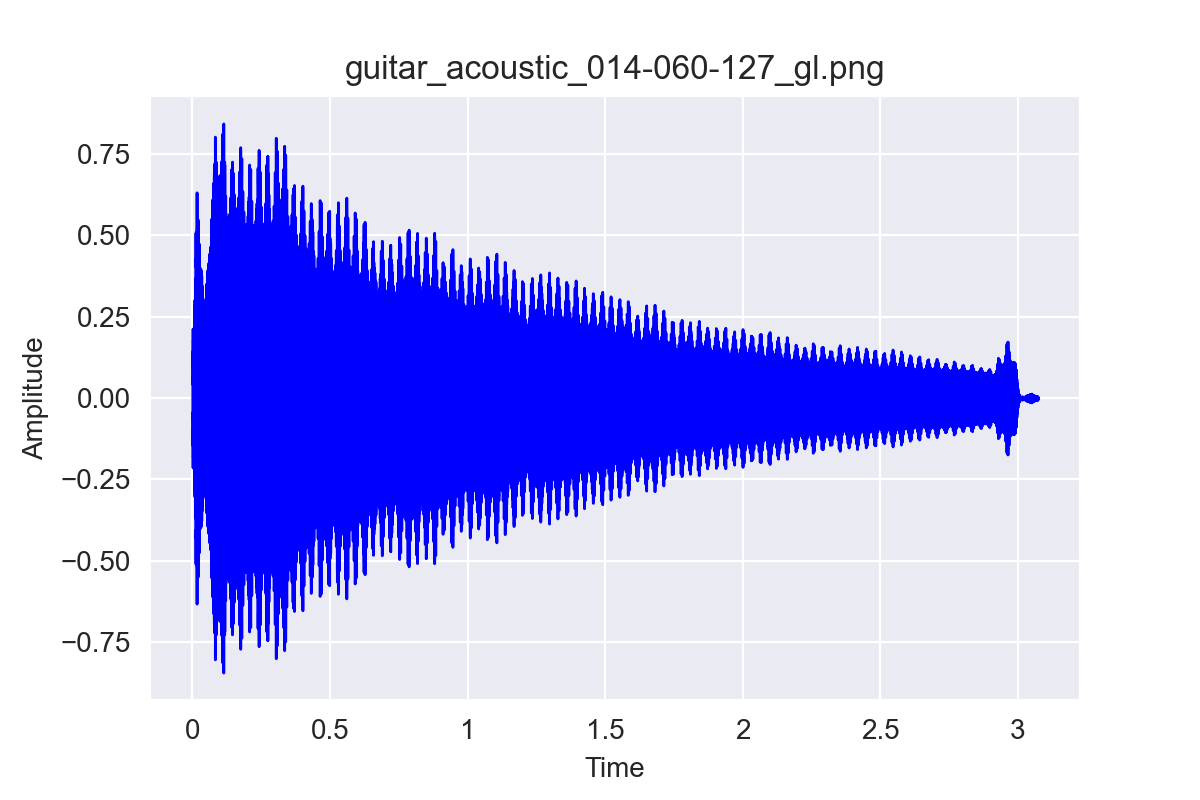
\includegraphics[width=0.55\textwidth]{images/appendix/mel_double_stride/guitar_acoustic_014-060-127_gl.png}}&
        \makebox{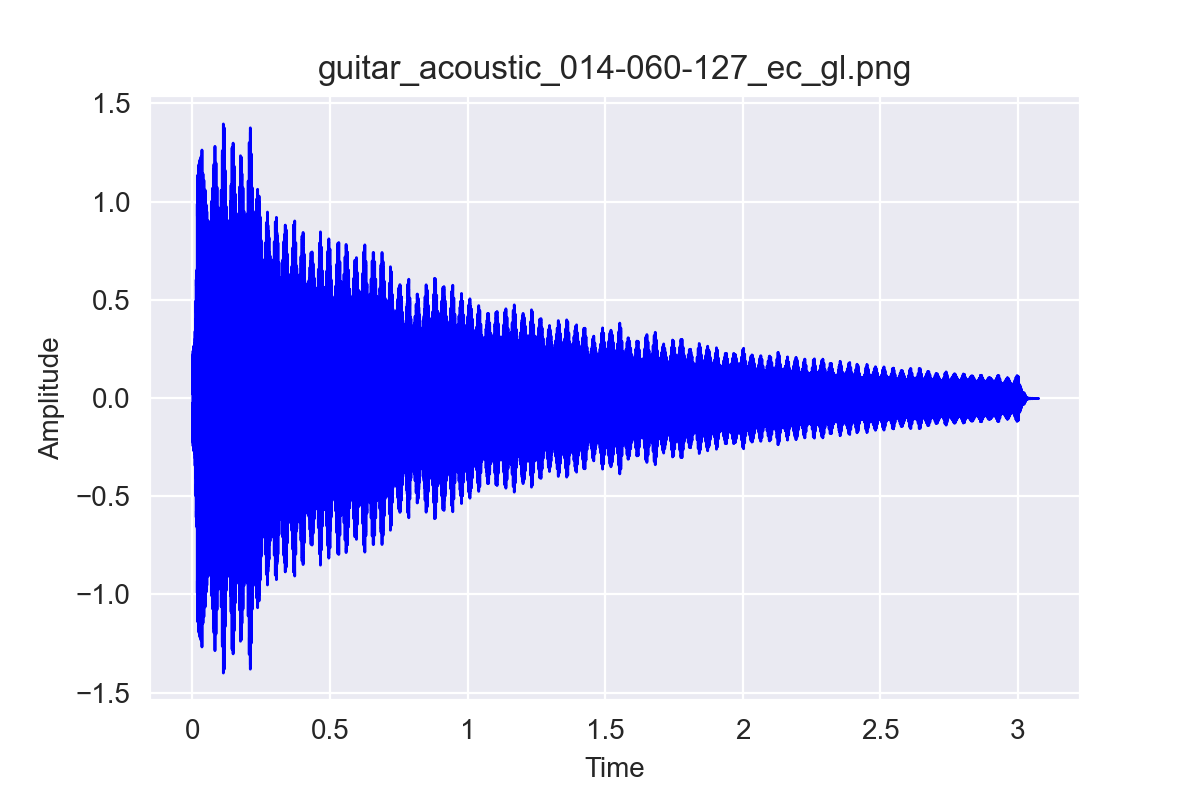
\includegraphics[width=0.55\textwidth]{images/appendix/mel_double_stride/guitar_acoustic_014-060-127_ec_gl.png}}\\
        (a) & (b)
    \end{tabular}}
    \caption{2D convolutional double-stride network (log-mel) - guitar acoustic output without post processing and Griffin Lim ~(a), output with post processing and Griffin Lim ~(b).}
    \label{fig:apx_mel_double_gf}
\end{figure}

\begin{figure}[htb!]
    \centering
    \captionsetup{justification=centering}
    \makebox[\textwidth][c]{\begin{tabular}{@{}cc@{}}
        \makebox{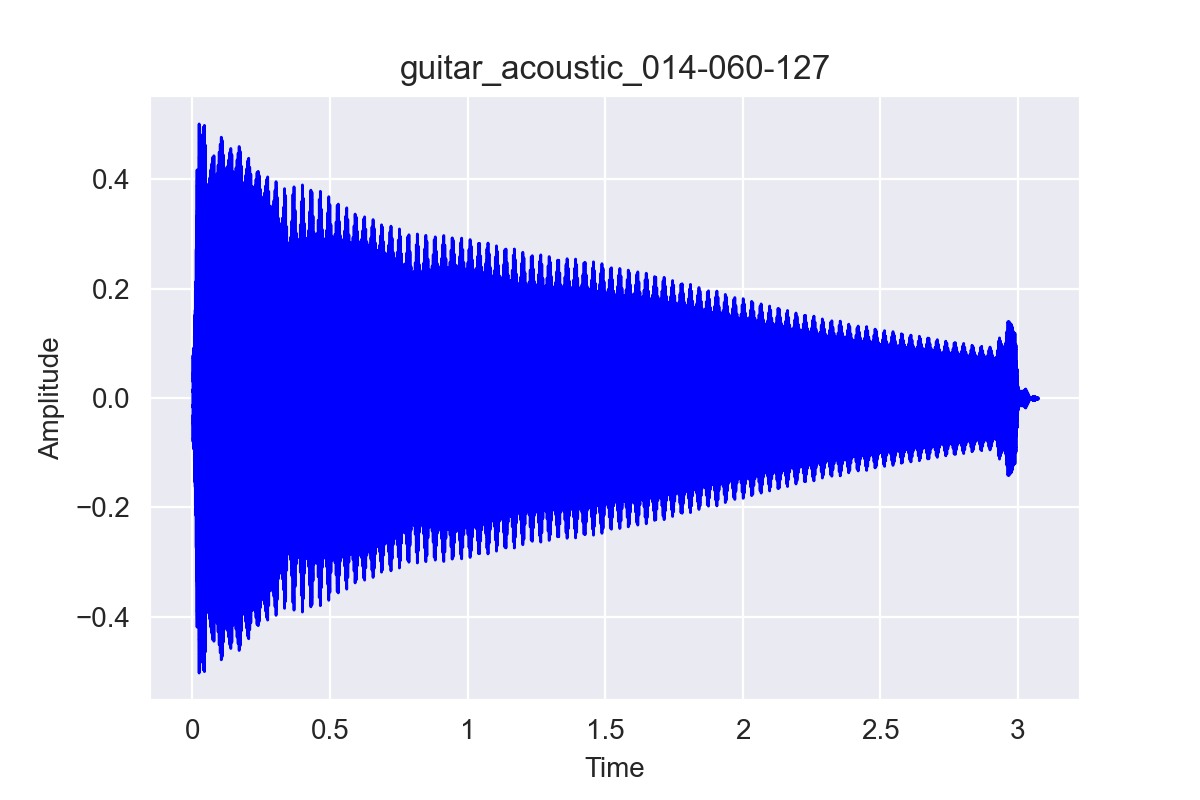
\includegraphics[width=0.55\textwidth]{images/appendix/mel_triple_stride/guitar_acoustic_014-060-127.png}}&
        \makebox{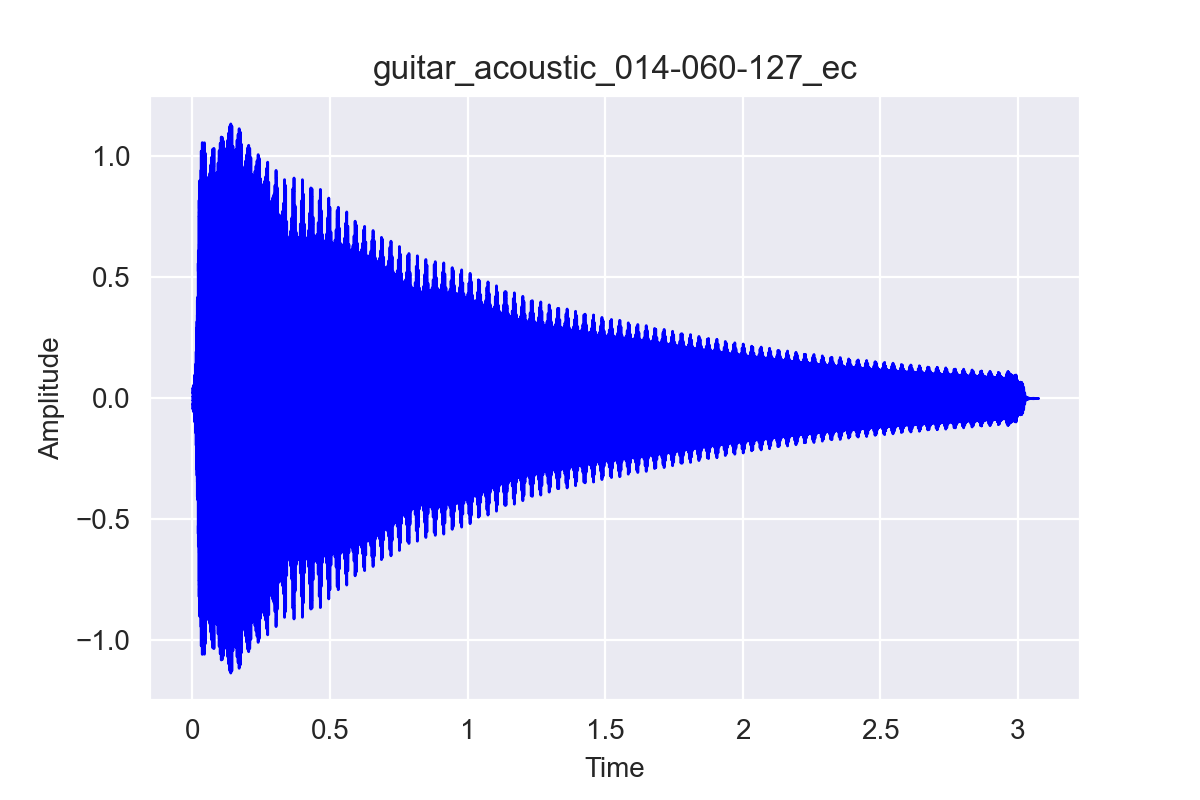
\includegraphics[width=0.55\textwidth]{images/appendix/mel_triple_stride/guitar_acoustic_014-060-127_ec.png}}\\
        (a) & (b)
    \end{tabular}}
    \caption{2D convolutional triple-stride network (log-mel) - guitar acoustic output without post processing ~(a), output with post processing ~(b).}
    \label{fig:apx_mel_triple_phase}
\end{figure}

\begin{figure}[htb!]
    \centering
    \captionsetup{justification=centering}
    \makebox[\textwidth][c]{\begin{tabular}{@{}cc@{}}
        \makebox{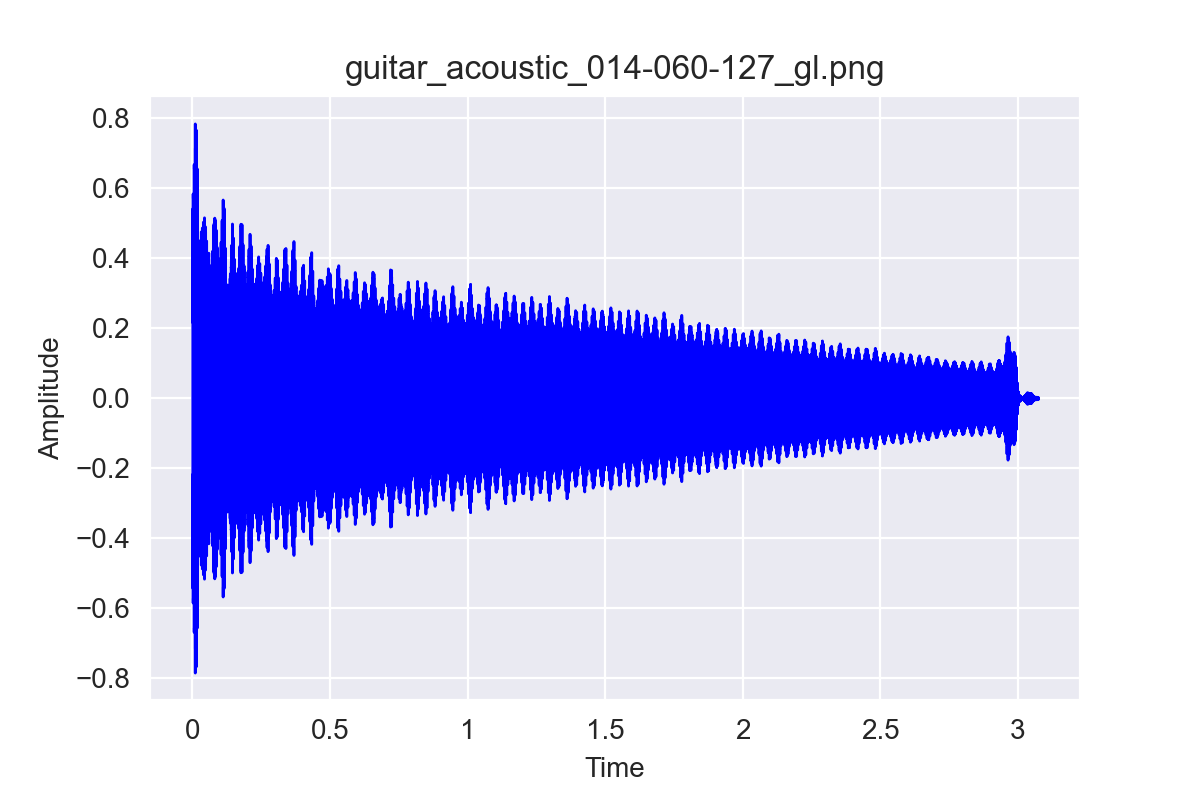
\includegraphics[width=0.55\textwidth]{images/appendix/mel_triple_stride/guitar_acoustic_014-060-127_gl.png}}&
        \makebox{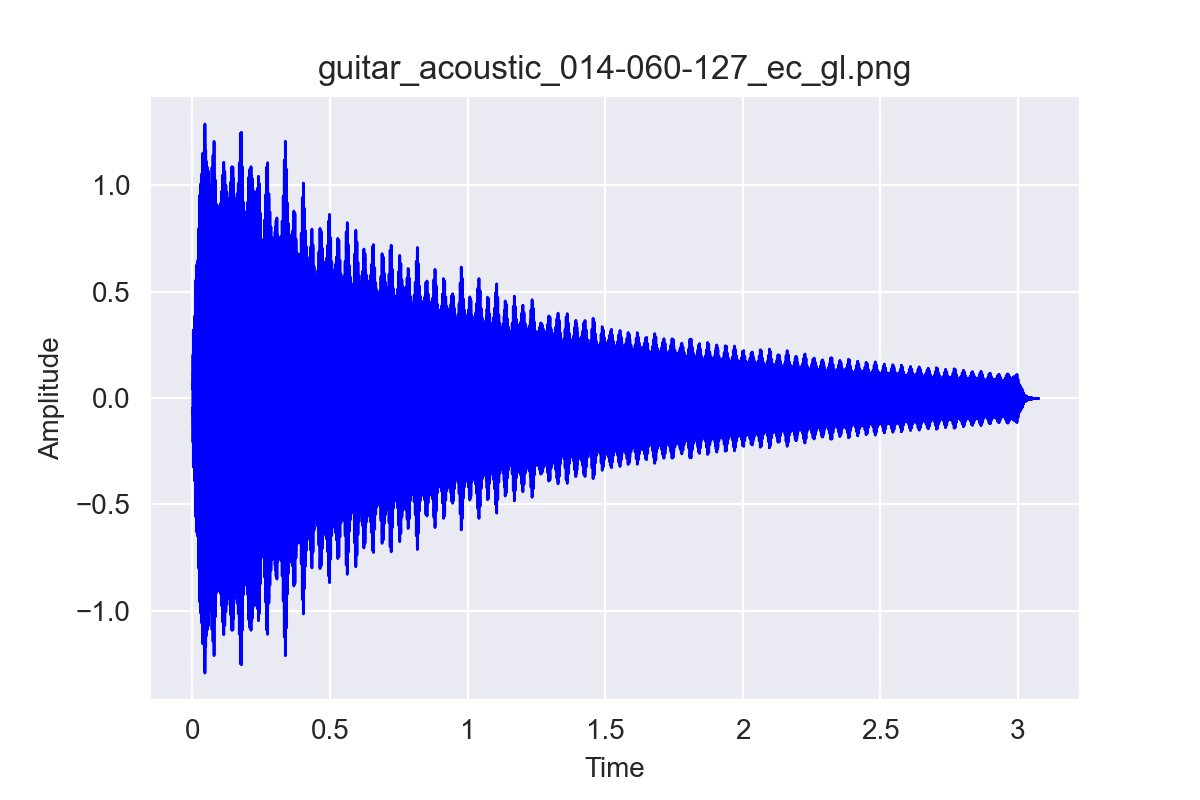
\includegraphics[width=0.55\textwidth]{images/appendix/mel_triple_stride/guitar_acoustic_014-060-127_ec_gl.png}}\\
        (a) & (b)
    \end{tabular}}
    \caption{2D convolutional triple-stride network (log-mel) - guitar acoustic output without post processing and Griffin Lim ~(a), output with post processing and Griffin Lim ~(b).}
    \label{fig:apx_mel_triple_gf}
\end{figure}